%-*-coding: utf-8-*-
\chapter{Решение задачи поиска кратчайшего расстояния от фиксированной вершины до всех остальных}
\label{chapSVD}

В данной главе описаны алгоритмы по решению классической задачи на графах --- поиску кратчайших расстояний от одной вершины до всех остальных. В первой части главы представлен обзор существующих решений задачи. Во второй части предложены разработанные мною параллельные модификации алгоритма Беллмана-Форда. В третьей части реализованные алгоритмы сравниваются и выявляются области их применимости.

\FloatBarrier
\section{Обзор существующих решений}

В данном разделе представлен краткий обзор предметной области --- последовательные и параллельные модификации алгоритма Беллмана-Форда.

\FloatBarrier
\subsection{Алгоритм Беллмана-Форда}

В контексте решения задачи поиска кратчайших расстояний от одной вершины до всех остальных существует два наиболее распространенных решения --- алгоритм Дейкстры и алгоритм Беллмана-Форда. Существует множество модификации алгоритма Дейкстры, которые в зависимости от используемой структуры данных работают $O(V^2+E)$, $O(E \log V)$ или $O(V \log V+E)$.\footnote{V --- количество вершин}\footnote{E --- количество ребер} Однако такие алгоритмы не работают на графах с отрицательным весом ребер. Классический алгоритм Беллмана-Форда работает на графах с произвольным весом ребер. Важным его недостатком является асимптотика --- $O(VE)$. Однако за счет возможности ранней остановки алгоритма и различных оптимизаций на практике на некоторых графовых структурах он может давать результаты, лучшие чем алгоритм Дейкстры. Именно по этой причине основной упор в работе делается на этот алгоритм. Также известны специализированные алгоритмы, такие как алгоритм A* и D*, которые оперирует большими специализированными графами и используют ряд эвристик для поиска расстояний. При этом в контексте наших исследований они затронуты не будут, а сосредоточимся мы именно на алгоритме Беллмана-Форда и его модификациях.   

В основе алгоритма лежит идея динамического программирования. После $k$ итерации алгоритма утверждается, что будут корректно посчитаны и обработаны пути длиной не более $k$. И после $V$ итерации расстояние до каждой из вершин посчитано корректно. Ниже приведен каноничный псевдокод алгоритма. 

\FloatBarrier
\begin{algorithm}
\caption{Классический алгоритм Беллмана-Форда}\label{bf_classic_seq}
\begin{algorithmic}[1]
\Procedure{ClassicBellmanFord}{$G,start$}
\State {$dist \gets \left\{ {\infty ... \infty}\right\}$}
\State {$dist[start] \gets 0$}
 
\For{$i = 0$ to $|G.vertices| - 1 $}
	\For{$e \in G.edges $}
		\State $dist[e.to] \gets \min(dist[e.to], dist[e.from] + e.w)$
	\EndFor
\EndFor
\State \textbf{return} $dist$
\EndProcedure
\end{algorithmic}
\end{algorithm}

\FloatBarrier
Кроме того, существует интересная модификация алгоритма, которая поддерживает на каждой итерации набор вершин, расстояние до которых изменилось на предыдущем шаге алгоритма. Из очевидных соображений мы имеем право рассматривать только эти и никакие другие вершины. Этот алгоритм на практике зачастую работает заметно быстрее, чем классическая версия. Однако в некоторых случаях он оказывается медленнее. Об этих особенностях подхода подробно описано в разделе, посвященному сравнению алгоритмов. Будем называть эту версию BFS-подобный Беллман-Форд (алгоритм \ref{bf_bfs_seq}). 

\FloatBarrier
\begin{algorithm}
\caption{BFS-подобный Беллман-Форд}\label{bf_bfs_seq}
\begin{algorithmic}[1]
\Procedure{BFSBellmanFord}{$G,start$}
\State $dist\gets \left\{ {\infty ... \infty}\right\}$
\State $dist[start] \gets 0$
\State $CurrentVertexSet \gets \left\{ {start}\right\}$\Comment{Набор вершин, расстояние до которых обновилось} 
\State $NextVertexSet \gets \emptyset$ 
\State {$step \gets 0$ }
\While {$step < |G.vertices|$ \algorithmicand \algorithmicnot $ CurrentVertexSet.empty()$}
	\State $step \gets step + 1$
	\State $NextVertexSet.clear()$
	
	\For{$v \in CurrentVertexSet$}
		\For{$e \in G.edgesFrom[v] $} \Comment{Исходящие ребра из текущей вершины} 
			\If {$dist[e.to] > dist[e.from] + e.w$} 
				\State $dist[e.to] \gets dist[e.from] + e.w$
				\State $NextVertexSet.insert(e.to)$								
			\EndIf
		\EndFor
	\EndFor
	
	\State $CurrentVertexSet \gets NextVertexSet$	
\EndWhile
\State \textbf{return} $dist$

\EndProcedure
\end{algorithmic}
\end{algorithm}


\FloatBarrier
\subsection{Обзор параллельных модификации Беллмана-Форда}

Большинство параллельных алгоритмов опираются на классическую реализацию алгоритма Беллмана-Форда и применяют различные методы для параллелизации внутреннго цикла релаксации ребер \cite{COHEN}\cite{GAURAV}. Кроме того, известны статьи, в которых описаны методы параллелизации BFS-подобной версии Беллмана-Форда \cite{LIGRA}. Мною предложенная BFS-подобная версия показала лучший результат, нежели существующий аналог. При этом для параллельных модификации классической версии были обозначены области применения и их преимущества и недостатки относительно BFS-подобной версии. Однако, в силу специфичности многих существующих решений и их зависимости от библиотек, на которых они основаны, мною предложенные параллельные версии классического Беллмана-Форда сравниваться с аналогами не будут. 


\FloatBarrier
\section{Параллельный алгоритм Беллмана-Форда}

В предыдущем разделе были рассмотрены классические алгоритмы поиска кратчайших путей в графе, а также существующие параллельные модификации. В этом разделе будут рассмотрены мною разработанные версии алгоритма Беллмана-Форда в контексте параллельных вычислений. Кроме того, будем использовать в каждом из алгоритмов идею ранней остановки --- если на текущем шаге ни одно из значений массива расстояний не изменилось, то имеем право выйти из основного цикла. В последующих подразделах будет представлено несколько версий алгоритма, а также их последующее сравнение и рекомендации по использованию.  

\FloatBarrier
\subsection{Параллелизация по ребрам вершины}

Прежде чем приступить к описанию параллельной версий выполним небольшую модификацию алгоритма. Будем для каждой вершины перебирать не исходящие ребра, а входящие. Это ход даст нам одно важное преимущество в контексте параллельных алгоритмов --- значение кратчайшего расстояния до каждой вершины теперь может изменять лишь один поток, тогда как раньше могли несколько, что увеличивало потенциальные проблемы с гонками за ресурс.

Первая версия алгоритма основана на параллельной обработке всех ребер, входящих в текущую вершины. Псевдокод, который уже использует идею из предыдущего абзаца, приведен ниже. Алгоритм, как и классическая версия, работает в худшем случае за $O(VE)$. 



\FloatBarrier
\begin{algorithm}
\caption{Параллельный Беллман-Форд по ребрам вершины}\label{bf_classic_par1}
\begin{algorithmic}[1]
\Procedure{BellmanFordPar1}{$G,start$}
\State $dist\gets \left\{ {\infty ... \infty}\right\}$
\State $dist[start] \gets 0$
 
\For{$i = 0$ to $|G.vertices| - 1 $}
	\State {$changed \gets $ \algorithmicfalse}
	\For{$v \in G.vertices $}
		\algrenewcommand\algorithmicfor{\textbf{parfor}}
		\State $minDist \gets dist[v]$

		\For{$e \in G.edgesTo[v] $} \Comment{Входящие ребра в текущую вершину} 
			\State $minDist \gets \min(minDist, dist[e.from] + e.w)$
		\EndFor	
					
		\If {$dist[v] > minDist$} 
			\State $dist[v] \gets minDist$ \Comment{Атомарно} 

			\State {$changed \gets $ \algorithmictrue}					
		\EndIf

		\algrenewcommand\algorithmicfor{\textbf{for}}

	\EndFor
	\If {\algorithmicnot $changed$} 
		\State \textbf{break}
	\EndIf

\EndFor
\State \textbf{return} $dist$
\EndProcedure
\end{algorithmic}
\end{algorithm}
\FloatBarrier

\begin{figure}[h]
\centering
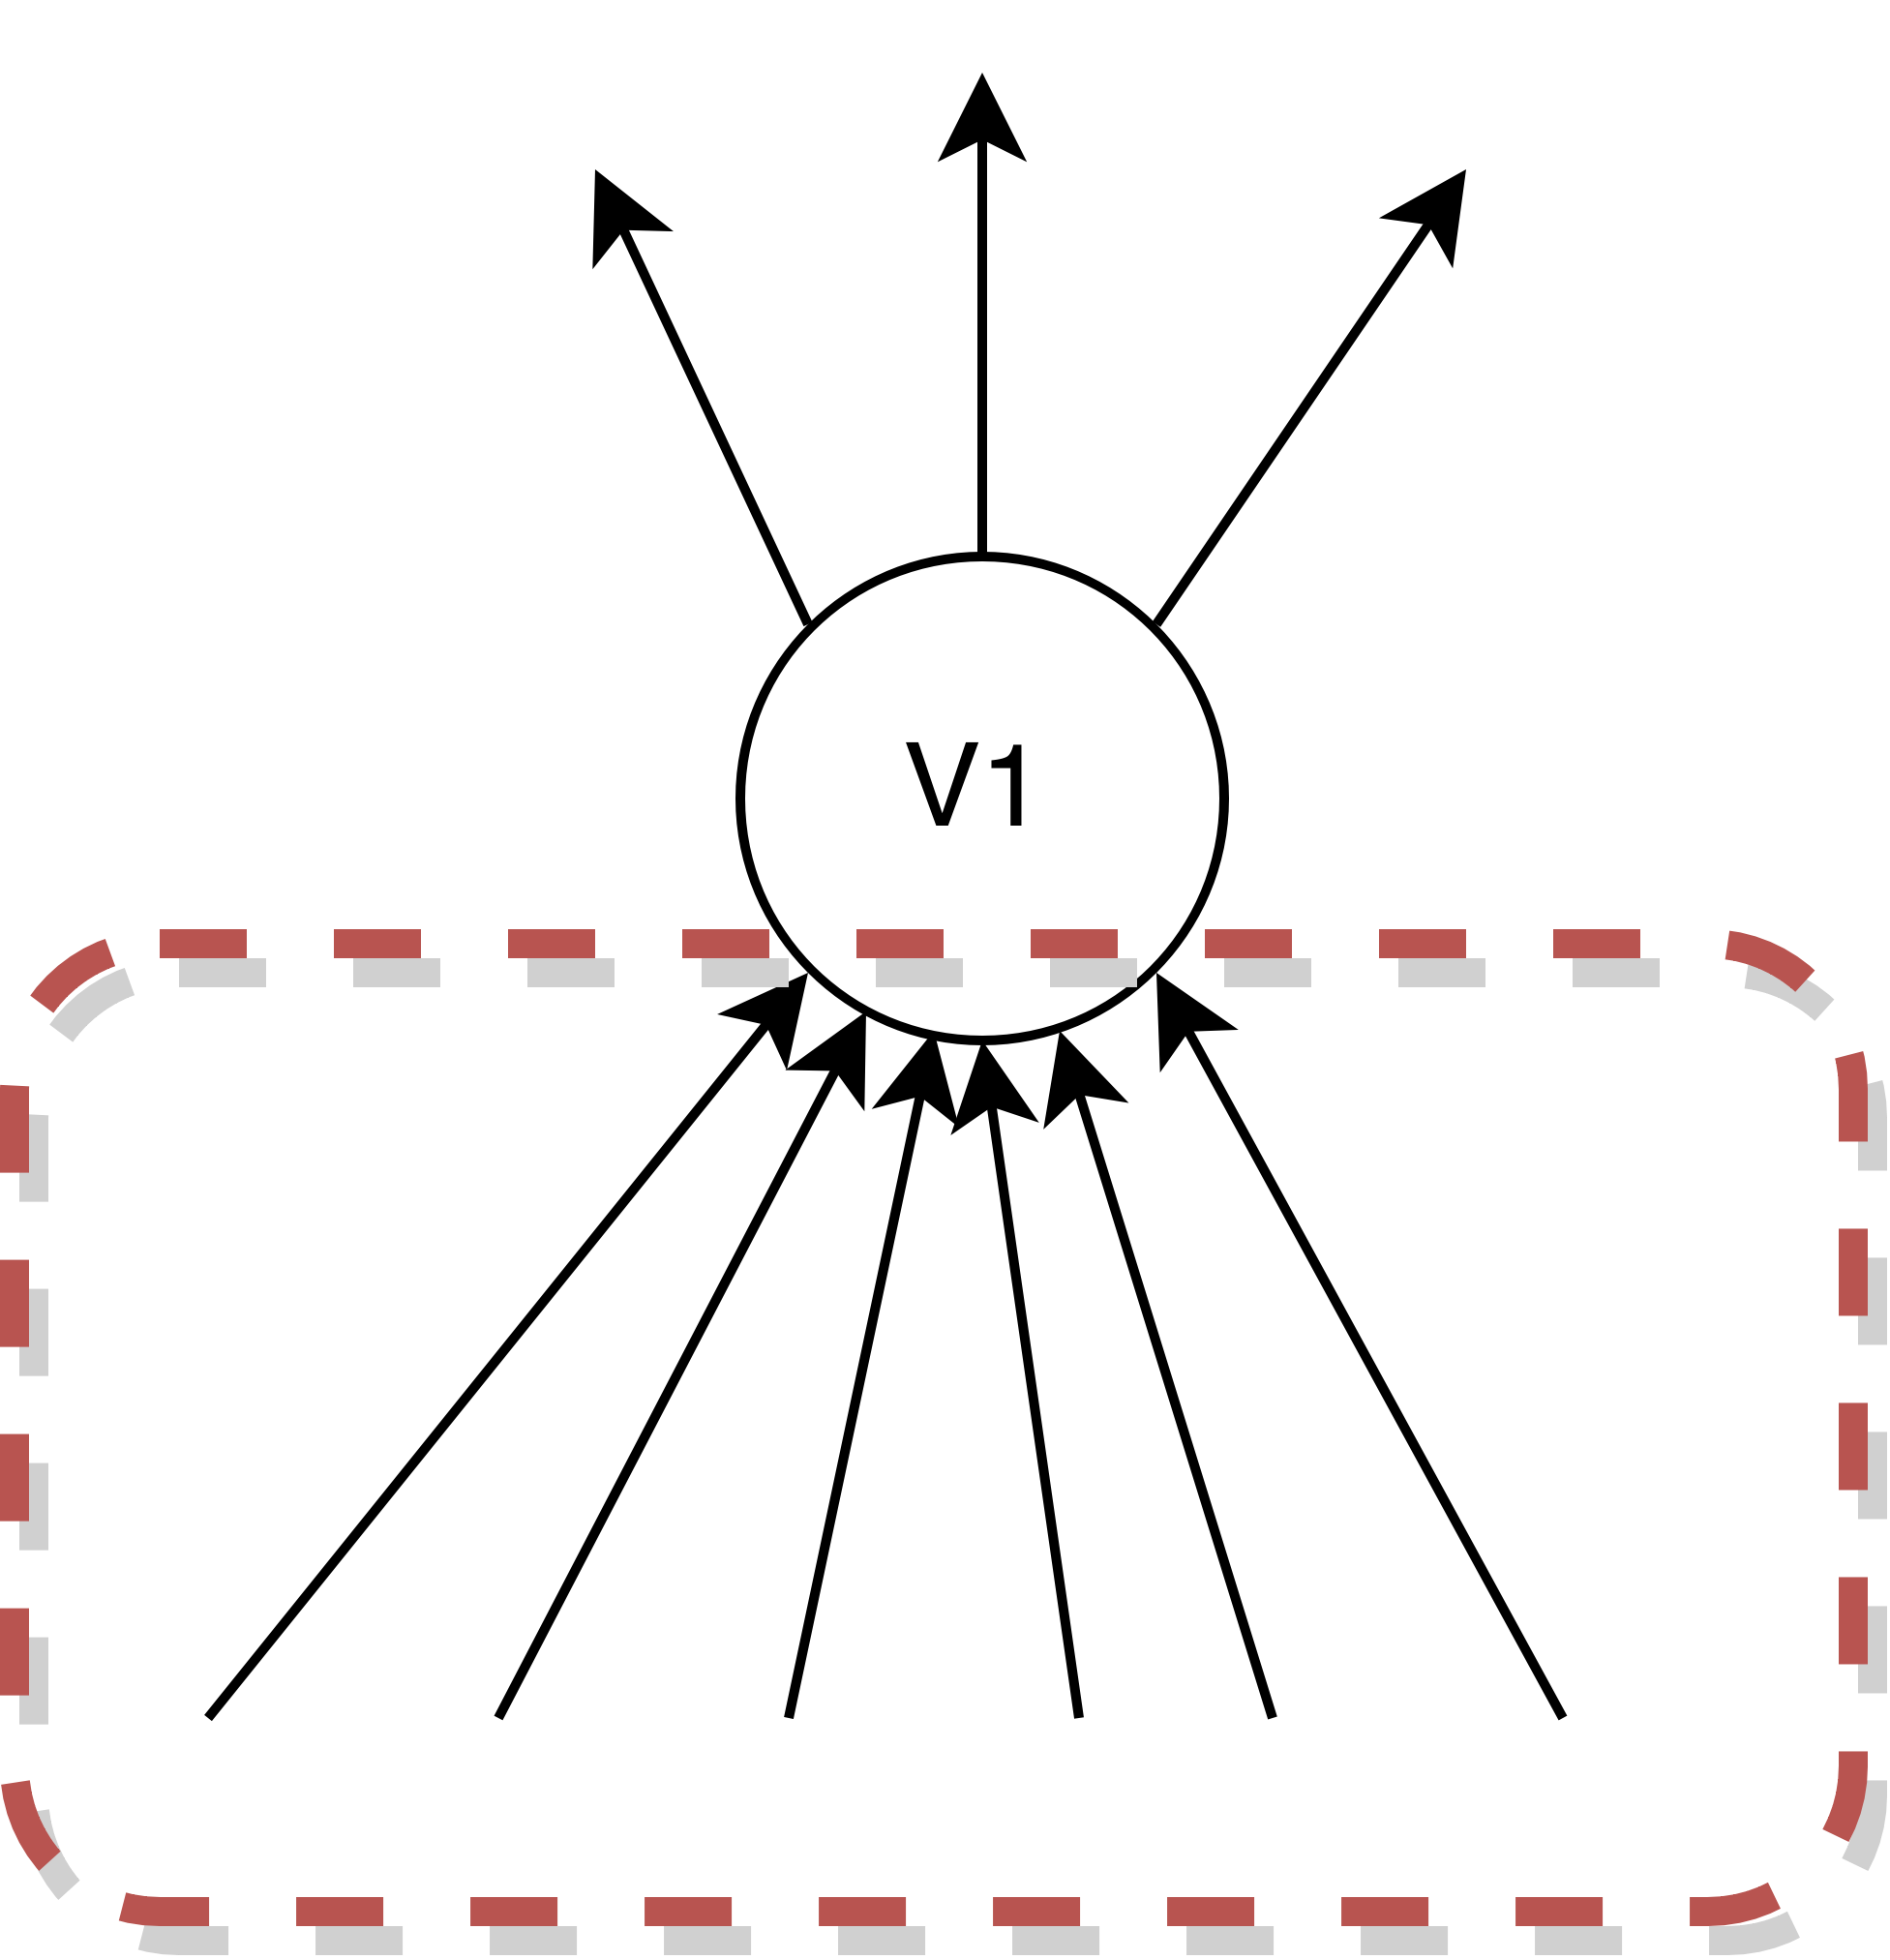
\includegraphics[width=0.4\textwidth]{img/bf_par_1.png}
\caption{Параллелизация по ребрам вершины}
\label{bf_par_1}
\end{figure}

\FloatBarrier
\subsection{Параллелизация по всем ребрам}
Идея второго алгоритма состоит в разбиений всего набора вершин на некоторые подмножества, каждое из которых будет обрабатываться отдельным процессором. При этом опять же, как и в предыдущем алгоритме, для каждой вершины будем рассматривать набор ребер, входящих в нее. 

Рассмотрим псеводкод алгоритма. Процесс поиска расстояний разбивается на два этапа. Рассмотрим каждый из этапов по отдельности.

На первом этапе мы строим разбиение всего множества вершин на подмножества, каждое из которых будет обрабатываться последовательно. Причем необходимо выполнить разбиение таким образом, чтобы суммарное количество входящих в вершины текущего подмножества ребер было не более $threshold$. Добиться этого можно с помощью рекурсивной функции $BuildPlan$, которая на текущем шаге находит с помощью двоичного поиска такую вершину текущего отрезка, которая разбивает множество входящих в вершины ребер примерно пополам. Далее индекс такой вершины запоминается в хэш-таблицу, ключом которой является пара индексов концов текущего отрезка. Для эффективной реализации двоичного поиска предпосчитаем частичные суммы для входящих ребер --- это необходимо, чтобы мы могли в двоичном поиске получать за $O(1)$ количество входящих ребер на некотором отрезке вершин. 

\FloatBarrier

\begin{figure}[h]
\centering
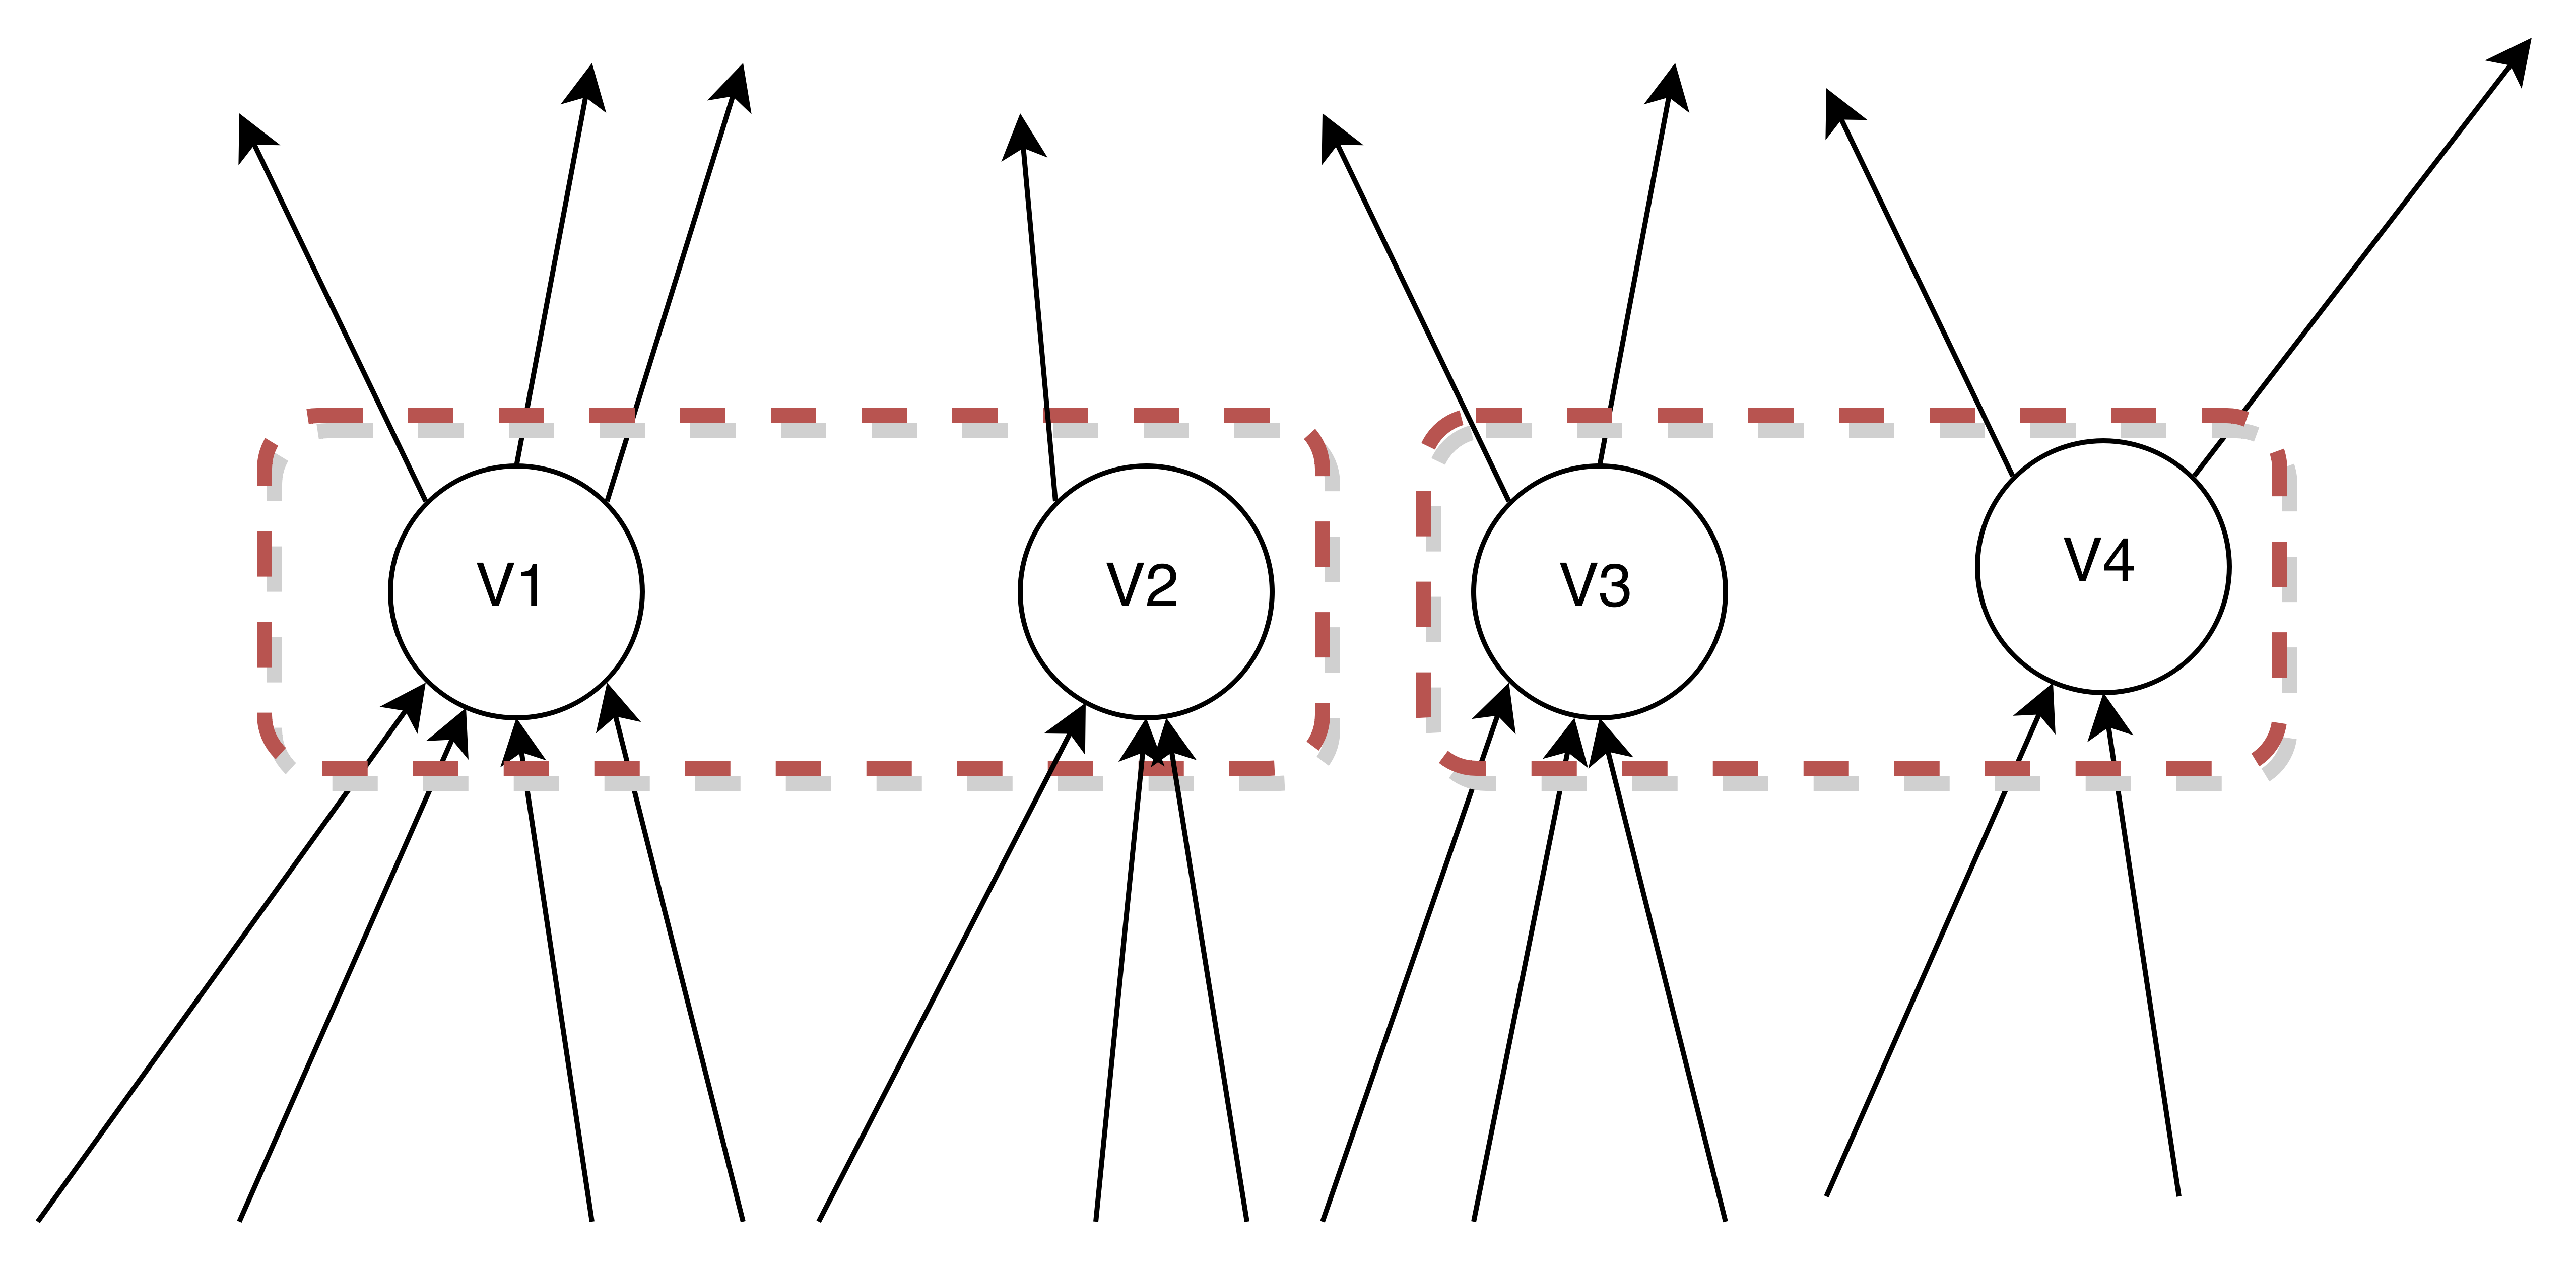
\includegraphics[width=0.8\textwidth]{img/bf_par_2_2.png}
\caption{Параллелизация по всем ребрам}
\label{bf_par_2_2}
\end{figure}

На втором этапе мы непосредственно вычисляем кратчайшие расстояния до вершин. Эта функция использует посчитанные раннее частичные суммы и полученную из функции $BuildPlan$ хэш-таблицу. На текущем шаге функция проверяет больше ли количество входящих ребер текущего отрезка значения $threshold$. Если значение оказывается меньше, то обработка ребер выполняется последовательно. Иначе, с помощью посчитанной на первом этапе хэш-таблицы выбирается индекс середины отрезка (в смысле числа входящих ребер) и параллельно запускается обработка двух подотрезков вершин. Операция выбора середины отрезка будет выполняться за $O(1)$ за счет хэш-таблицы.

Алгоритм также как и предыдущая версия работает в худшем случае за $O(VE)$, однако он имеет значительно большую практическую пользу. Эта тема будет подробно рассмотрена позднее в подразделе «Сравнение подходов». 
\FloatBarrier
\begin{algorithm}[H]
\caption{Параллельный Беллман-Форд по всем ребрам}\label{bf_classic_par2}
\begin{algorithmic}[1]
\Procedure{BellmanFordPar2}{$G,start$}
\State $dist\gets \left\{ {\infty ... \infty}\right\}$
\State $dist[start] \gets 0$
\State {$prefsum \gets $ prefix sum by vertices incoming degree} 
\State {$planMap \gets $ empty map}
\State \Call {BuildPlan}{$prefsum$, 0, |$G.vertices$|, planMap}

\For{$i = 0$ to $|G.vertices| $}	
	\If {\algorithmicnot \Call {ProcessLayer}{$G, dist, planMap, prefsum, 0, |G.vertices|$}} 
		\State \textbf{break}
	\EndIf
		
\EndFor
\State \textbf{return} $dist$
\EndProcedure

\State 
\Procedure{BuildPlan}{$prefsum, startV, endV, resultMap$}  
\State $edgesNumber \gets prefsum[endV] - prefsum[startV]$
\If {$edgesNumber < threshold$} 
	\State $midV \gets $ Бинарным поиском по массиву prefsum находим индекс вершины $midV$, что $prefsum[midV]-prefsum[startV] \approx prefsum[endV]-prefsum[midV]$
	\State $resultMap[startV][endV] \gets midV$ 
	\State \Call {BuildPlan}{$prefsum, startV, midV, resultMap$} 
	\State {\Call {BuildPlan}{$prefsum, midV, endV, resultMap$}} 
\EndIf

\State \textbf{return} $resultMap$
\EndProcedure

\State 
\Procedure{ProcessLayer}{$G, dist, planMap, prefsum, startV, endV$}  
\State $edgesNumber \gets prefsum[endV] - prefsum[startV]$
\If {$edgesNumber < threshold$} 
	\State {\textbf{return} {\Call {ProcessVerticesSequentially}{$G, dist, startV, endV$}}}
\Else	
	\State $midV \gets planMap[startV][endV]$ 
	\State {$changed \gets $ \algorithmicfalse}

	\State {$changed = changed $ \algorithmicor \Call {ProcessLayer}{$G, dist, planMap, prefsum, startV, midV$}}
	\State {$changed = changed $ \algorithmicor \Call {ProcessLayer}{$G, dist, planMap, prefsum, midV, endV$}}
	\State \textbf{return} $changed$
\EndIf

\EndProcedure

\State 
\Procedure{ProcessVerticesSequentially}{$G, dist, startV, endV$}  

\State {$changed \gets $ \algorithmicfalse}
\For{$v = startV$ to $endV - 1 $}
		\State $minDist \gets dist[v]$

		\For{$e \in G.edgesTo[v] $} \Comment{Входящие ребра в текущую вершину} 
			\State $minDist \gets \min(minDist, dist[e.from] + e.w)$
		\EndFor	
					
		\If {$dist[v] > minDist$} 
			\State $dist[v] \gets minDist$ \Comment{Атомарно} 

			\State {$changed \gets $ \algorithmictrue}					
		\EndIf
\EndFor
\State \textbf{return} $changed$

\EndProcedure

\end{algorithmic}
\end{algorithm}

\FloatBarrier
\subsection{Параллелизация BFS-версии}
Предыдущие две версии были основаны на параллелизации классической версии Беллмана-Форда. В основе следующего алгоритма лежит BFS-подобный Беллман-Форд (алгоритм \ref{bf_bfs_seq}). В качестве основы для параллельной версии такого алгоритма был взят параллельный обход в ширину, предложенный Умутом Акаром и Майком Рэйни \cite{FRONTIERSEARCH}. 


Ключевым моментом в алгоритме является использованием структуры данных Frontier. Она подробно рассмотрена в статье Умута Акара и Майка Рэйни. Здесь же приведено краткое ее описание, основные принципы работы и интерфейс. Frontier представляет из себя некоторый набор ребер. При этом он поддерживает операции разделения множества пополам, слияния множеств, добавления ребер вершины и итерирования по ребрам. При этом  операции слияния и разбиения выполняются асимптотически за $O(\log n)$, добавление ребер вершины происходит за константу, а итерирование за константу для каждого ребра. Такая асимптотика достигается за счет лежащей в основе Bootstrapped Chunked Sequence \cite{CHUNKEDSEQ}, которая представляет из себя последовательность, где каждому элементу сопоставляется его вес. И операций слияния и разбиения выполняются в соответсвии с этими весами и выполняются за $O(\log n)$. Более подробное описание Bootstrapped Chunked Sequence приведено в указанной раннее статье. 

Кроме того, в алгоритме используются важная возможность библиотеки для параллельных вычислений PASL \cite{PASL} (является альтернативой известного решения Cilk \cite{CILK}) --- взаимодействие между несколькими потоками. А именно каждый из потоков может понимать нуждаются ли в «помощи» другие потоки. И в случае положительного ответа он может «поделиться» данными для вычислений. 

Таким образом, псевдокод алгоритма представлен ниже. В основе главной функции алгоритма $HandleFrontier$ лежит следующая идея. В процессе обработки текущего $CurFrontier$ мы во-первых узнаем нуждается ли другой процессор в данных для вычисления. Если да, то делимся в случае достаточного количества ребер. Иначе обрабатываем некоторое константное значени ребер ($pollingCutoff$) и запускаем процесс снова. Обратим внимание, что в нем использованы упомянутые ранее возможности библиотеки PASL --- функции $hasIncomingQuery$ и $rejectQuery$. 

\begin{algorithm}[H]
\caption{Параллельный BFS-подобный Беллман-Форд}\label{bf_bfs_par}
\begin{algorithmic}[1]
\Procedure{BellmanFordPar3}{$G,start$}
\State $dist\gets \left\{ {\infty ... \infty}\right\}$
\State $layerForVertex\gets \left\{ {-1 ... -1}\right\}$ \Comment{Номер последнего уровня, в котором посетили вершину} 
\State $dist[start] \gets 0$
\State $layerForVertex[start] \gets 0$
\State {$Frontier \gets \left\{ {G.edgesFrom(start)}\right\}$}\Comment{Исходящие ребра текущего множества } 

\For{$layer = 1$ to $|G.vertices| $}	
	\State $NextFrontier \gets \emptyset$

	\State {$Frontier \gets $  {\Call {HandleFrontier}{$Frontier, NextFrontier, layer, dists, layerForVertex$}}} 
	
	\If { $Frontier.empty()$} 
		\State \textbf{break}						
	\EndIf
		
		
\EndFor
\State \textbf{return} $dist$
\EndProcedure
\State

\Procedure{HandleFrontier}{$CurFrontier, NextFrontier, layer, dists, layerForVertex$}
\While {\algorithmicnot $CurFrontier.empty()$}
	\If {$hasIncomingQuery()$}
		\If {$CurFrontier.nbEdges() \leq cutoff$}
			\State $rejectQuery()$			
		\Else		
			\State $NewCurFrontier \gets \emptyset$
			\State $NewNextFrontier \gets \emptyset$
			\State $CurFrontier.split(NewCurFrontier)$
			\State \begin{varwidth}[t]{\linewidth}fork2(\par
        \hskip\algorithmicindent {\Call {HandleFrontier}{$CurFrontier, NextFrontier, layer, dists, layerForVertex$}},\par
        \hskip\algorithmicindent {\Call {HandleFrontier}{$NewCurFrontier, NewNextFrontier, layer, dists, layerForVertex$}});
      \end{varwidth}
 			\State $NextFrontier.split(NewNextFrontier)$

		\EndIf
		
	\EndIf
	\State Frontier.iterNumber(pollingCutoff, updateFunction(from, to, weight, layer, dists, layerForVertex))
\EndWhile
\EndProcedure
\State
\Procedure{UpdateFunction}{$from, to, weight, layer, dists, layerForVertex, NextFrontier$}
\If {{\Call {TryToUpdateDistance}{$to, dists[from] + weight, dists$}}} 

	\If {{\Call {TryToSetVisited}{$to, layer, layerForVertex$}}} 
		\State $NextFrontier.pushEdgesOf(to)$
	\EndIf
	
\EndIf
\EndProcedure
\State
\Procedure{TryToSetVisited}{$vertex, layer, layerForVertex$}
\If {\algorithmicnot $layerForVertex[vertex] = layer$} 
	\State \textbf{return} {$cas(layerForVertex[vertex], layerForVertex[vertex], layer)$ }  
\EndIf
\State \textbf{return} {\algorithmicfalse}  
\EndProcedure
\State
\Procedure{TryToUpdateDistance}{$vertex, candidate, dists$}
\State \textbf{return} {$writeMin(dists[vertex], candidate)$} \Comment Атомарный минимум 
\EndProcedure

\end{algorithmic}
\end{algorithm}

\begin{figure}[h]
\centering
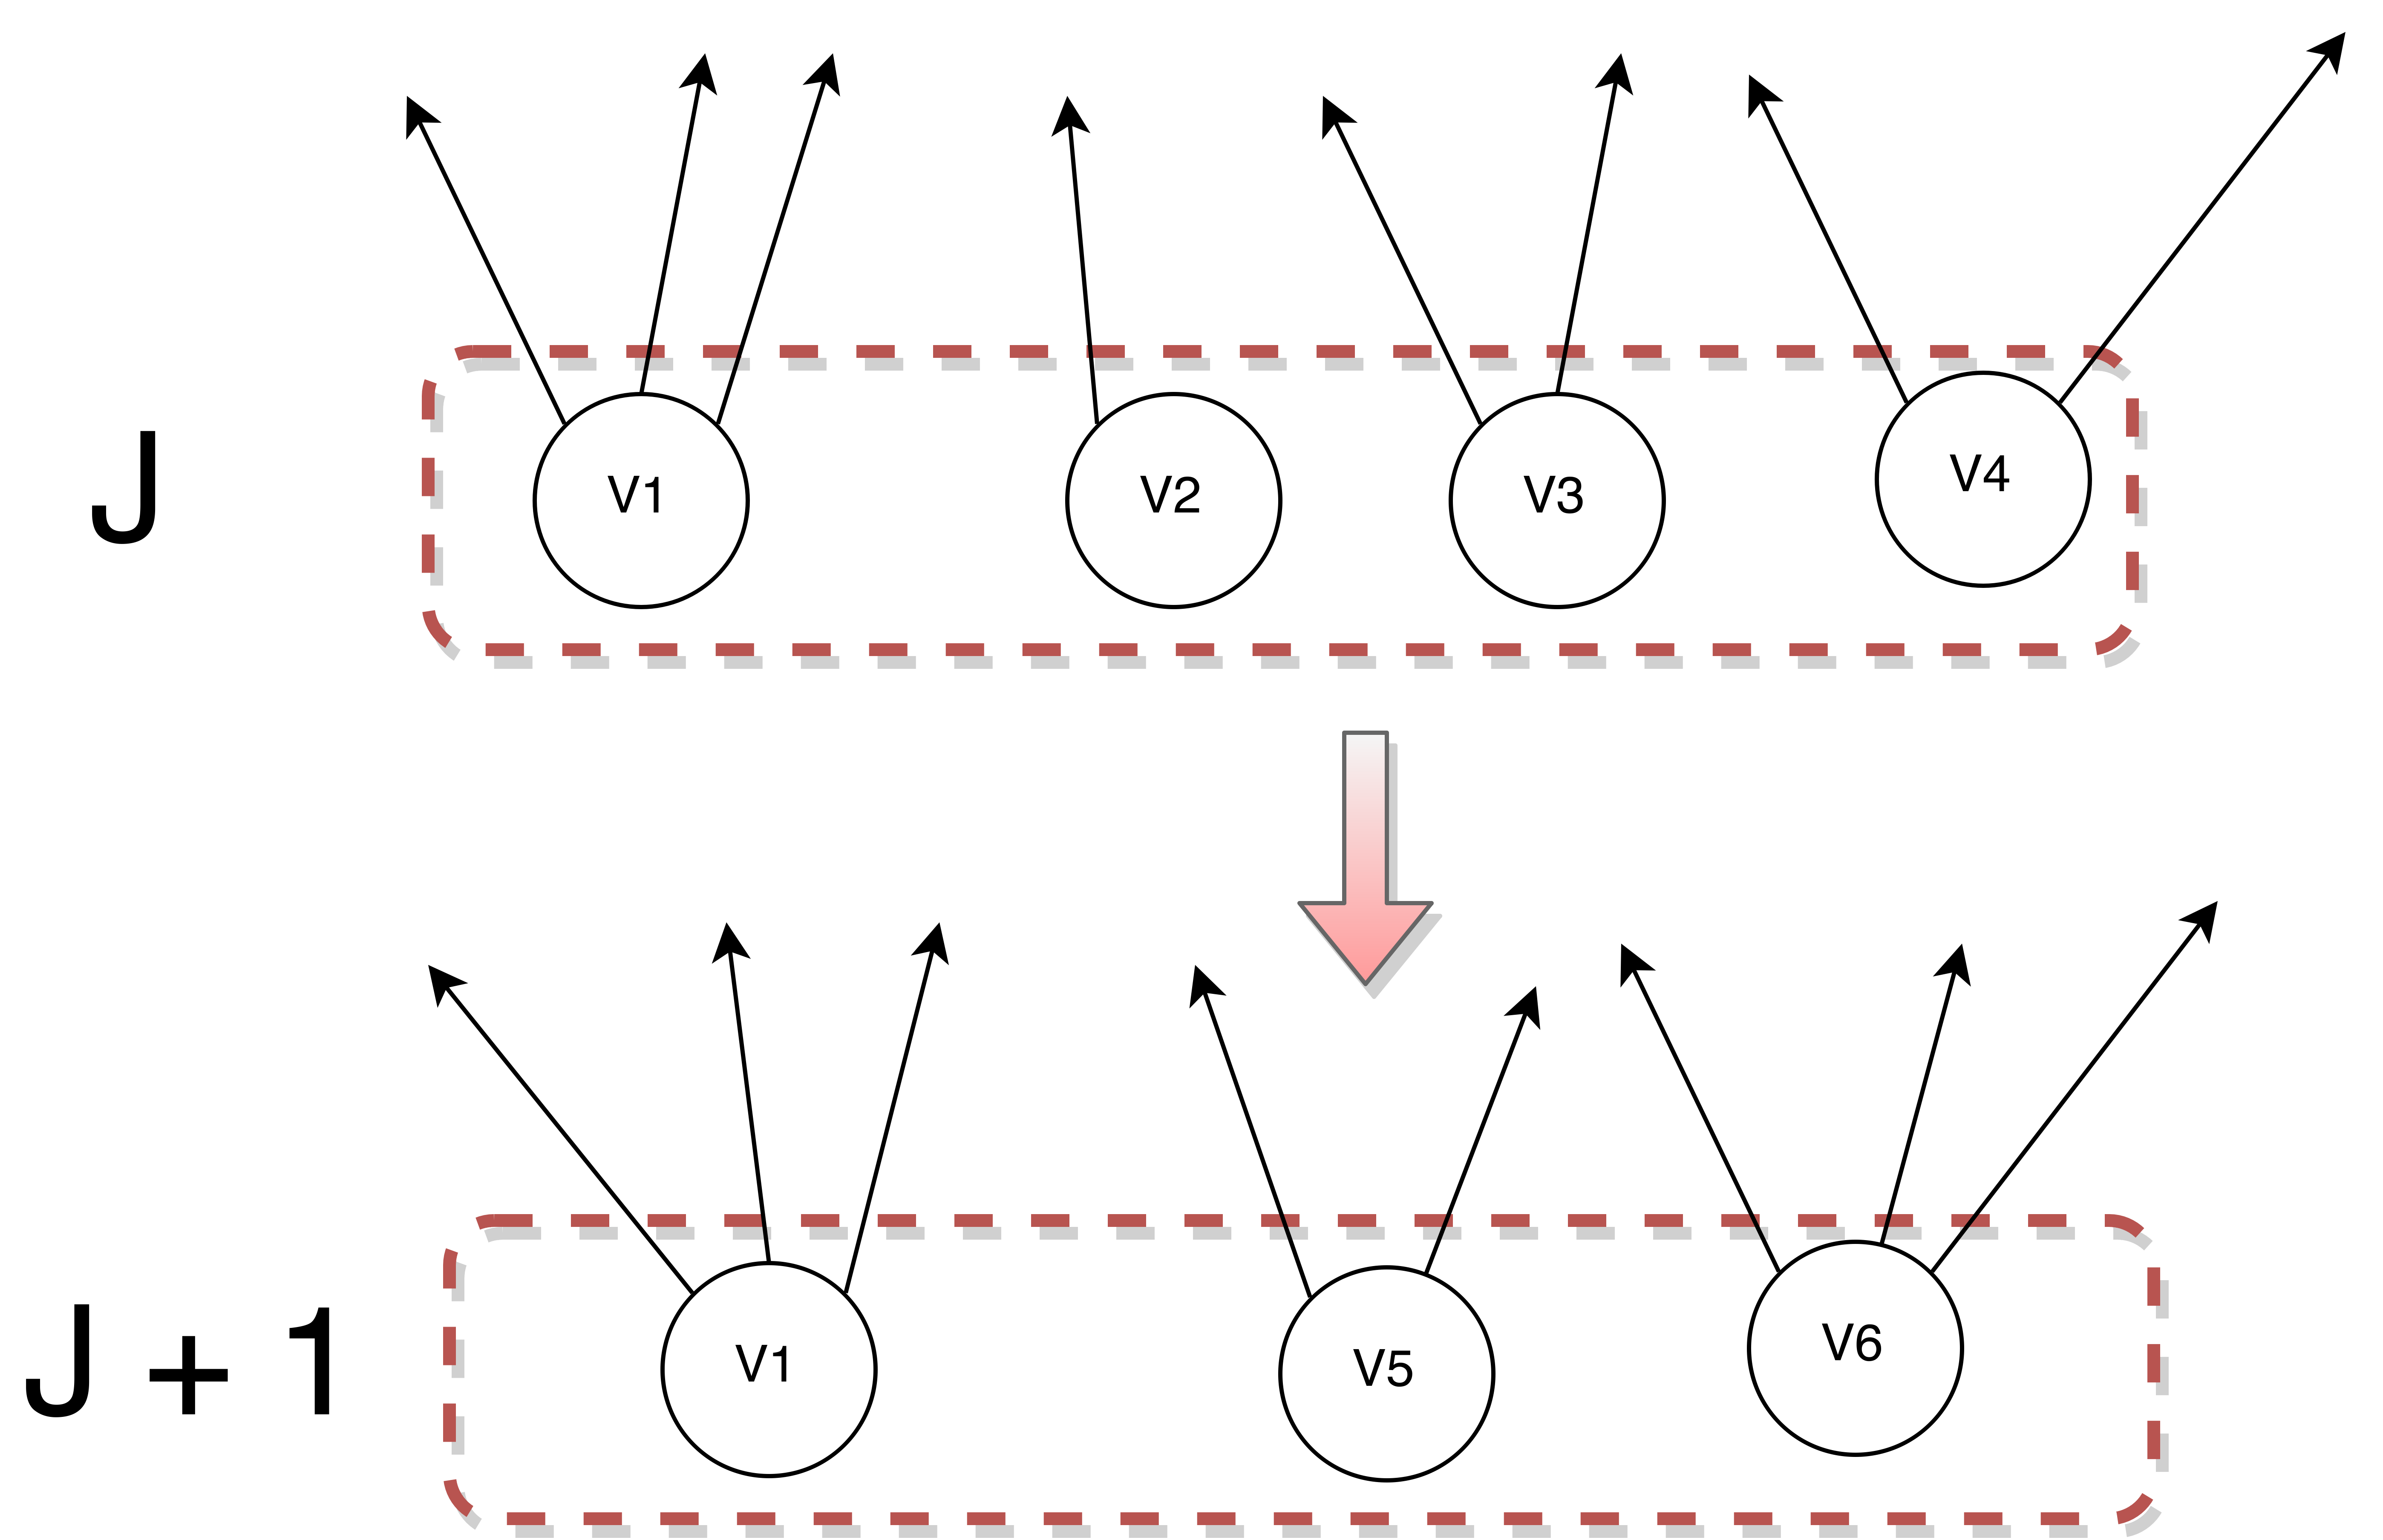
\includegraphics[width=0.75\textwidth]{img/bf_par_3.png}
\caption{Параллелизация BFS-версии}
\label{bf_par_3}
\end{figure}

\FloatBarrier
\subsection{Сравнение подходов}
Несмотря на то, что все три алгоритма в худшем случае имеют одну асимптотику  $O(VE)$, каждый из вышеизложенных подходов имеет свои особенности, что позволяет каждому из них конкурировать друг с другом на некоторых типах графов. Рассмотрим эти особенности.

С первого взгляда может показаться, что алгоритм \ref{bf_classic_par1} имеет лишь одни недостатки --- он наименьшим образом по сравнению с последующими задействует все процессоры и при этом асимптотически равен остальным двум. Однако рассмотрим внимательнее каноничный алгоритм Беллмана-Форда и запустим его на плотном графе, где для каждого ребра верно, что индекс вершины источника меньше индекса вершины назначения (будем называть такое ребро лексикографически отсортированным). В этом случае каноничной версии достаточно будет сделать лишь две итерации внешнего цикла, поскольку на каждой итерации внутреннего цикла значение расстояния для текущей вершины будет корректно посчитано (очевидно доказывается по принципу математической индукции). Иными словами, в этом случае алгоритм работает за $O(V + E)$. Так как количество итерации третьего алгоритма в подобных графах может быть значительным и размер текущей очереди может быть большим, а второму же алгоритму на таких графах хорошая способность параллелиться будет только вредить --- она будет заметно увеличивать число итераций внешнего цикла, то в таких случаях последние два алгоритма работают хуже первого.   

Но, очевидно, что в большинстве случаев последние два алгоритма будут показывать лучшие результаты. Сравним эти два подхода. Алгоритм, основанный на обходе в ширину, заметно сокращает количество вершин для обработки в пределах каждой итерации, что дает заметное преимущество на разреженных графах по сравнению с алгоритмом \ref{bf_classic_par2}, где на каждом шаге обрабатываются все ребра. Однако на плотных графах количество таких вершин значительно, что негативно сказывается на производительности алгоритма в силу множественных и трудоемких операций с памятью. То есть такой подход показывает себя не с лучшей стороны в подобных графах. Кроме того, в случае с графами с циклами отрицательного веса даже в случае разреженного графа размер текущего Frontier может быть велик. Это достигается в том случае, если количество вершин, из которых достижим цикл отрицательного веса велико. Однако провести такой анализ графа в общем случае не является простой задачей, то будем рекомендовать к использованию алгоритм \ref{bf_classic_par2} при наличии в графе ребер отрицательного веса.

\FloatBarrier
\subsection{Тестирование}

Для подтверждения вышеприведенных рассуждений все вышеизложенные подходы были реализованы на основе уже раннее упомянутой библиотеки для параллельных вычислений PASL. В качестве языка программирования использовался C++. Тестирование производилось на ряде графов на 40-ядерной машине Intel с поддержкой hyper-threading \cite{HYPERTHREADING} с доступной оперативной памятью 256GB. 

Алгоритмы тестировались на различных графовых структурах, которые перечислены в Таблице \ref{bf_algo_comparison}. 
\FloatBarrier
\begin{table}[H]
\centering
\caption{Описание входных графов}

\begin{tabular}{c | c | c | l}  
\multicolumn{4}{l}{\footnotesize \textit{fraction} - Доля лексикографически отсортированных ребер (ребра вида $V_i \rightarrow V_{i+j}$) }\\
\hline
Название & Вершины & Ребра & Описание\\
\hline\hline
Complete TS & 7071 & 24995985 & Полный граф с fraction = 1 (TopSorted)\\  
Complete + & 3162 & 9995082 & Полный граф с положительным весом ребер \\  
Complete - & 3162 & 9995082 & Полный граф с случайным весом ребер \\  
BalancedTree F & 8388607 & 8388608 & Сбалансирование дерево с fraction = F \\  
SquareGrid + & 2499561 & 4999122 & Квадратная решетка с положительными ребрами \\  
SquareGrid - & 2499561 & 4999122 & Квадратная решетка с случайными ребрами \\  
RandomSparse 0.5+ & 2500000 & 25000000 & \pbox{9cm}{Случайный разреженный граф с положительными ребрами и fraction = 0.5\\}  \\  
RandomSparse 0.5- & 2500000 & 25000000 & \pbox{9cm}{Случайный разреженный граф с любыми ребрами и fraction = 0.5\\}  \\  
RandomSparse 0.96+ & 2500000 & 25000000 & \pbox{9cm}{Cлучайный разреженный граф с положительными ребрами и fraction = 0.96\\} \\  
RandomDense 0.5+ & 5000 & 25000000 & \pbox{9cm}{Случайный плотный граф с положительными ребрами и fraction = 0.5\\}  \\  
RandomDense 0.5- & 5000 & 25000000 & \pbox{9cm}{Случайный плотный граф с любыми ребрами и fraction = 0.5\\}  \\  
RandomDense 0.96+ & 5000 & 25000000 & \pbox{9cm}{Случайный плотный граф с положительными ребрами и fraction = 0.96\\}  \\  
\hline

\end{tabular}

\label{bf_algo_comparison}
\end{table}
\FloatBarrier
Средние значения времени исполнения каждой версии алгоритма на описанных графах представлены в таблице \ref{graph_description}. В тех случаях, когда время исполнения алгоритма было сильно выше, чем у аналогов (значение $\infty$ в таблице), выполнение алгоритма прерывалось.
\begin{table}[H]
\centering
\caption{Результаты измерений производительности}
\begin{tabular}{l|ccc|cc|cc|ccc|ccc}  
\hline
Алгоритм & \multicolumn{3}{c}{Complete} & \multicolumn{2}{c}{BalancedTree} & \multicolumn{2}{c}{SquareGrid} & \multicolumn{3}{c}{RandomSparse} & \multicolumn{3}{c}{RandomDense}\\
& TS & + & - & 0.5 & 1 & + & - & 0.5+  & 0.5- & 0.96+ & 0.5+ & 0.5- & 0.96+\\
\hline\hline
3 & 2.43 & 4.65 & $\infty$ & 116.31 & 9.04 & 5.49 & 13.40 & $\infty$ & $\infty$ & 24.35 & $\infty$ & $\infty$ & 5.01 \\  
4 & 5.17 & 0.18 & 10.84 & 3.59 & 3.08 & 5.92 & 7.10 & 2.77 & 14.68 & 2.42 & 0.48  & 6.38  & 0.46 \\
5 & 44.63 & 0.37 & 23.55 & 0.44 & 0.31 & 4.42 & 0.58 & 0.59 & 22.59 & 0.48  & 0.60  & 10.25 & 0.71 \\
Ligra & 49.13 & 0.30 & 26.11 & 0.55 & 0.50 & 8.15 & 1.21 & 0.58 & 25.19 & 0.54  & 1.12  & 14.15 & 1.20 \\
\hline
\end{tabular}

\label{graph_description}
\end{table}

\FloatBarrier
\section{Выводы}

Из таблиц видно, что наши ожидания относительно применимости конкретных подходов оправдались. Первый из алгоритмов работает лучше на узком спектре графов с высоким $fraction$ (доля лексикографически отсортированных ребер) и высокой средней степенью вершины, второй хорошо работает на плотных графах и графах с отрицательным весом ребер, третий же заметно лучше остальных на разреженных графах.

Кроме того, параллельный BFS-подобный Беллма-Форд оказался во многих ситуациях лучше аналога из библиотеки Ligra. Это прежде всего объясняется высокой производительностью работы структуры данных Frontier. Соответсвующее сравнение параллельных обходов в ширину, приведенное в работе Умута Акара \cite{FRONTIERSEARCH}, это еще раз подтверждает, поскольку эта модификация Беллмана-Форда во многом очень похожа на классический обход в ширину. 

Таким образом сделав простой анализ структуры графа мы сможем выбрать необходимый эффективный алгоритм для поиска кратчайшего пути. 
\FloatBarrier
